\section{Methodology and Experiment Setup}
\label{sec:methodology}
In this section, we will discuss in detail about umderlying working priniciples of SSD and different evaluation setups.
\subsection{Classifier Description}
We have initally attempted to train the system with simple unigram (bag of words), bigram, and tigram language model trained with $70\%$ of the tweets and testing with randomly selected $30\%$ of the tweets. For this binary classification task, we habe used SVM \cite{libsvm} with linear kernel and different ensemble techniques of boosting and bagging. Since we have a wide variety of features, we experimented with various ensemble learning techniques and found that LogitBoost performed best
empirically for boosting and bagging with SVM performed best for bagging technique. We used the Weka implementation of LogitBoost \cite{Friedman98} and EnsembleSVM for bagging \cite{ensembleSVM} to train a classifier using various combinations of features. We have used Decision Stumps as a base classifier in LogicBoost and ran boosting for 100 iterations. Furthermore, 
we have used SVM as a base classifier in bagging and ran bagging for 100 iterations. Training time of ensemble techniques were around $20$ hours in 8GB quadcore 3.2GHZ Ubuntu machine compared to around $1$ hour in SVM.

\subsection{Experiment Setup}

Fig. \ref{fig:infrastructure} shows the infrastructure of the whole system, which is divided into four parts: crawling module, parsing module, feature extracting module and sarcasm classifying module.

In the crawling module, we have developed a distributed crawling platform to collect a large-scale dataset from Twitter. The open-source tool Tweepy\cite{tweepy} was run on multiple machines in parallel, and all data will be centrally managed by the master node.

Raw tweets collected by the crawling module will be fed into the parsing module. The tool ark-twitter-nlp\cite{tweetnlp} was used to do tokenizing and POS tagging. After obtaining POS tagged tweets, TweeboParser\cite{kong2014dependency} will further run syntactic parsing which will generate syntactic dependency tree for each tweet. Named entity recognition was done by the tool in developed by Ritter et al\cite{Ritter11}\cite{Ritter12}. We applied sentiment analysis by utilizing the online machine learning framework Datumbox\cite{datumbox}. Due to the rate limit of this framework, we also created multiple parallel machine nodes to speed up sentiment analysis.

Parsed tweets are the input of the feature extracting module. We developed three feature extractors to extract corresponding features. After obtaining all tweet features, we are able to run the sarcasm classifying module, in which we used three classifiers, SVM with linear kernel, logitboosting with decision stump and bagging with SVM. 

\begin{figure}[htpb]
\centering
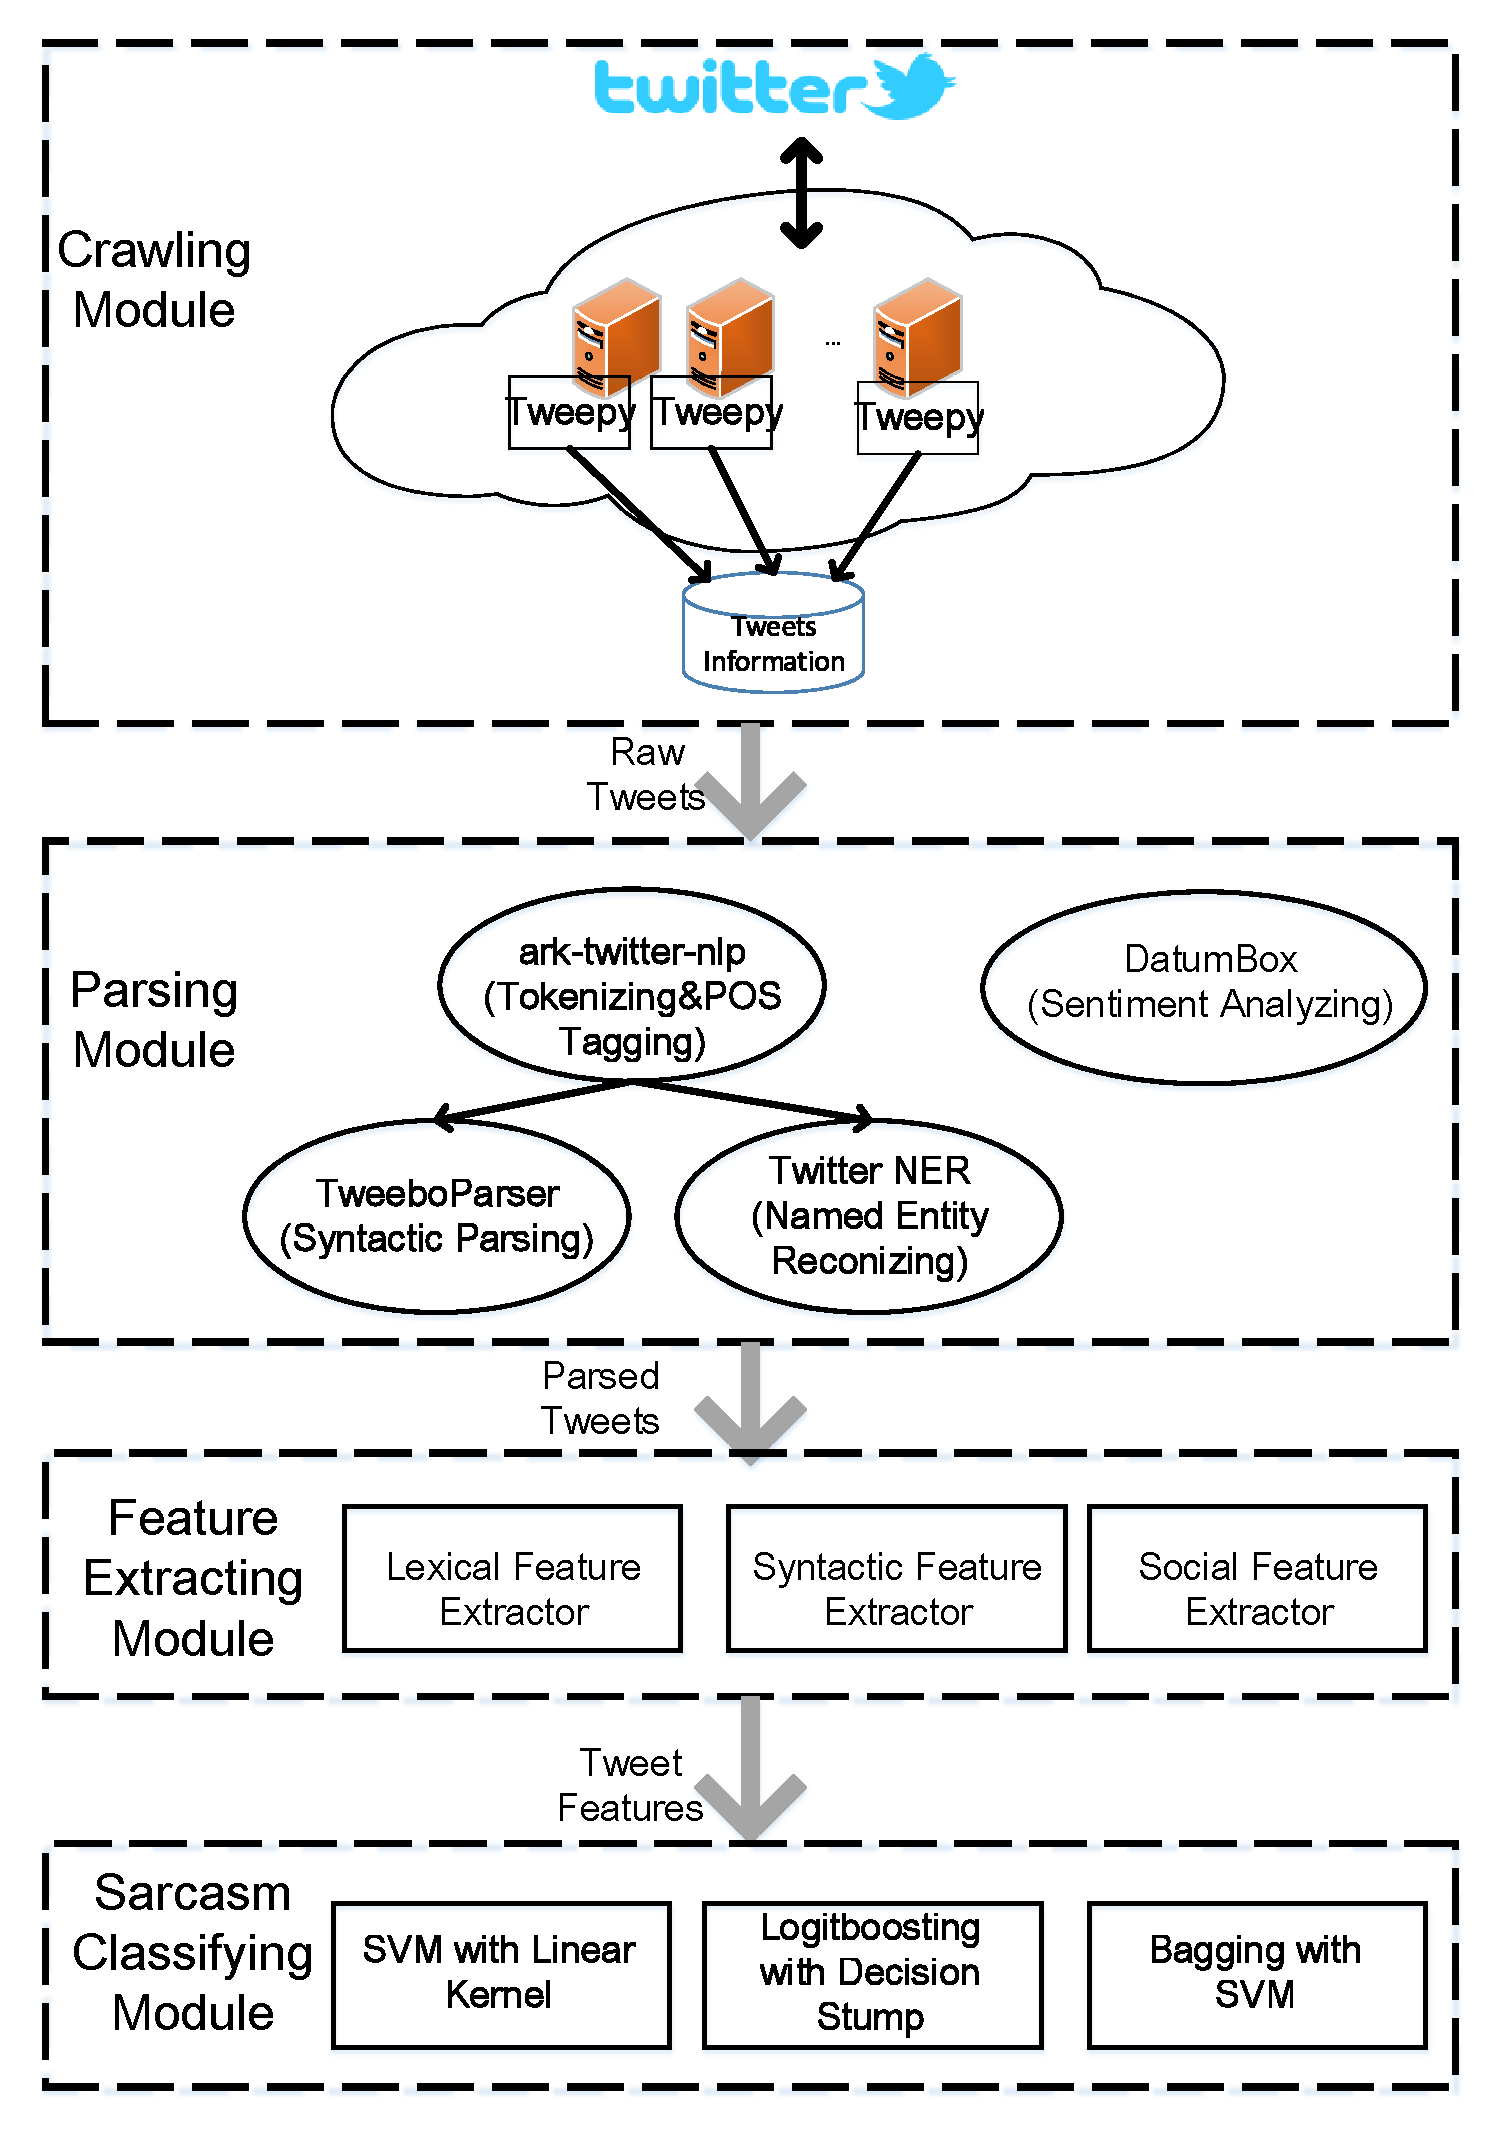
\includegraphics[scale=0.3]{infrastructure.eps}
\caption{The infrastructure of system setup.}
\label{fig:infrastructure}
\end{figure}
